\documentclass{article}\usepackage[]{graphicx}\usepackage{xcolor}
\usepackage{lineno}
\linenumbers

%% maxwidth is the original width if it is less than linewidth
%% otherwise use linewidth (to make sure the graphics do not exceed the margin)
\makeatletter
\renewcommand{\thetable}{A\arabic{table}}

\renewcommand{\thefigure}{A\arabic{figure}}
\def\maxwidth{ %
  \ifdim\Gin@nat@width>\linewidth
    \linewidth
  \else
    \Gin@nat@width
  \fi
}
\makeatother

\definecolor{fgcolor}{rgb}{0.345, 0.345, 0.345}
\newcommand{\hlnum}[1]{\textcolor[rgb]{0.686,0.059,0.569}{#1}}%
\newcommand{\hlstr}[1]{\textcolor[rgb]{0.192,0.494,0.8}{#1}}%
\newcommand{\hlcom}[1]{\textcolor[rgb]{0.678,0.584,0.686}{\textit{#1}}}%
\newcommand{\hlopt}[1]{\textcolor[rgb]{0,0,0}{#1}}%
\newcommand{\hlstd}[1]{\textcolor[rgb]{0.345,0.345,0.345}{#1}}%
\newcommand{\hlkwa}[1]{\textcolor[rgb]{0.161,0.373,0.58}{\textbf{#1}}}%
\newcommand{\hlkwb}[1]{\textcolor[rgb]{0.69,0.353,0.396}{#1}}%
\newcommand{\hlkwc}[1]{\textcolor[rgb]{0.333,0.667,0.333}{#1}}%
\newcommand{\hlkwd}[1]{\textcolor[rgb]{0.737,0.353,0.396}{\textbf{#1}}}%

\usepackage{framed}
\makeatletter
\newenvironment{kframe}{%
 \def\at@end@of@kframe{}%
 \ifinner\ifhmode%
  \def\at@end@of@kframe{\end{minipage}}%
  \begin{minipage}{\columnwidth}%
 \fi\fi%
 \def\FrameCommand##1{\hskip\@totalleftmargin \hskip-\fboxsep
 \colorbox{shadecolor}{##1}\hskip-\fboxsep
     % There is no \\@totalrightmargin, so:
     \hskip-\linewidth \hskip-\@totalleftmargin \hskip\columnwidth}%
 \MakeFramed {\advance\hsize-\width
   \@totalleftmargin\z@ \linewidth\hsize
   \@setminipage}}%
 {\par\unskip\endMakeFramed%
 \at@end@of@kframe}
\makeatother

\definecolor{shadecolor}{rgb}{.97, .97, .97}
\definecolor{messagecolor}{rgb}{0, 0, 0}
\definecolor{warningcolor}{rgb}{1, 0, 1}
\definecolor{errorcolor}{rgb}{1, 0, 0}
\newenvironment{knitrout}{}{} % an empty environment to be redefined in TeX

\usepackage{alltt}
\IfFileExists{upquote.sty}{\usepackage{upquote}}{}
\begin{document}

\section*{Additional files}

  In the main text of this manuscript, we showed the fitting and simulating results for Cat 1. Here, we have the adjusted BIC emission distribution comparisons, adjusted BIC across all FMM and HMM models, diurnal step lengths and autocorrelation plots for Cat 2, 14, and 15. Table A1 gives the name of panther ID (Cat ID) in Institutional Repository at the University of Florida (IR@UF), \cite{kerk2015hidden}, and number of observations for each panther. 
  
  
\begin{table}[h!]
\caption{Cat ID and number of observations; ID numbers are given matching
those shown by van de Kerk et al. 2015 and those 
in the data located at the UF Institutional repository (IR@UF).}
\begin{tabular}{cccc}
  \hline
  & van de Kerk 2015  & IR@UF   & Number of Observations\\ \hline
  & 130 & 1 & 10286\\
  & 131 & 2  & 9458\\
  & 48 & 14  & 14645\\
  & 94  & 15   & 10250\\ \hline
\end{tabular}
\end{table}
  
\newpage


















\begin{knitrout}
\definecolor{shadecolor}{rgb}{0.969, 0.969, 0.969}\color{fgcolor}\begin{figure}
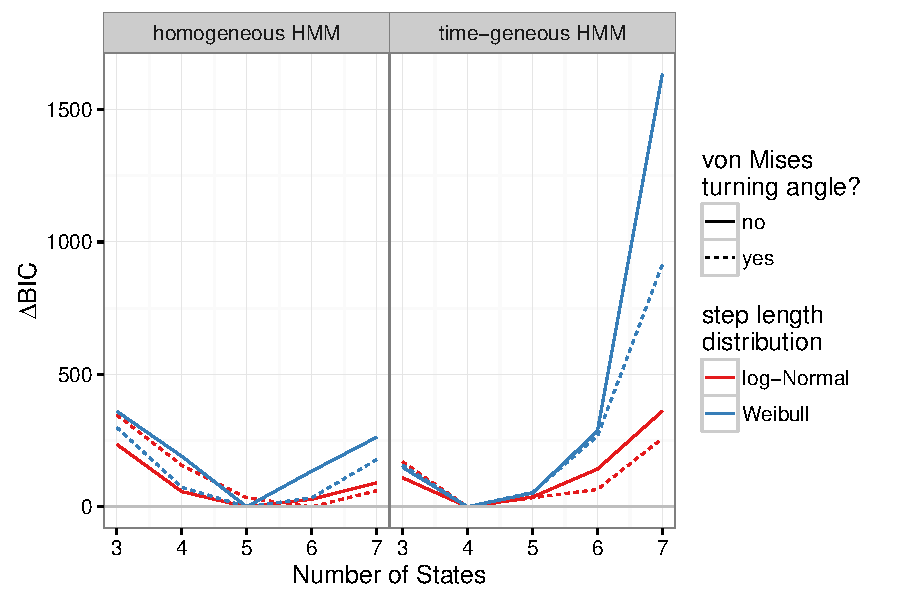
\includegraphics[width=\maxwidth]{figure/BICred_plot2-1} \caption{Cat 2: Comparison of BIC-optimal state predictions for homogeneous transition HMMs (left panel) and heterogeneous transition HMMs (right panel) with different emission complexities on panther data. Solid line represents univariate response/emission HMMs (without turning angles) and dotted line represents multivariate response HMMs (including turning angles with von-Mises distribution). Red lines represents log-normal step-length distribution and blue lines represents Weibull step-length distribution.}
\label{fig:BICred_plot2}
\end{figure}


\end{knitrout}

\clearpage
\begin{knitrout}
\definecolor{shadecolor}{rgb}{0.969, 0.969, 0.969}\color{fgcolor}\begin{figure}
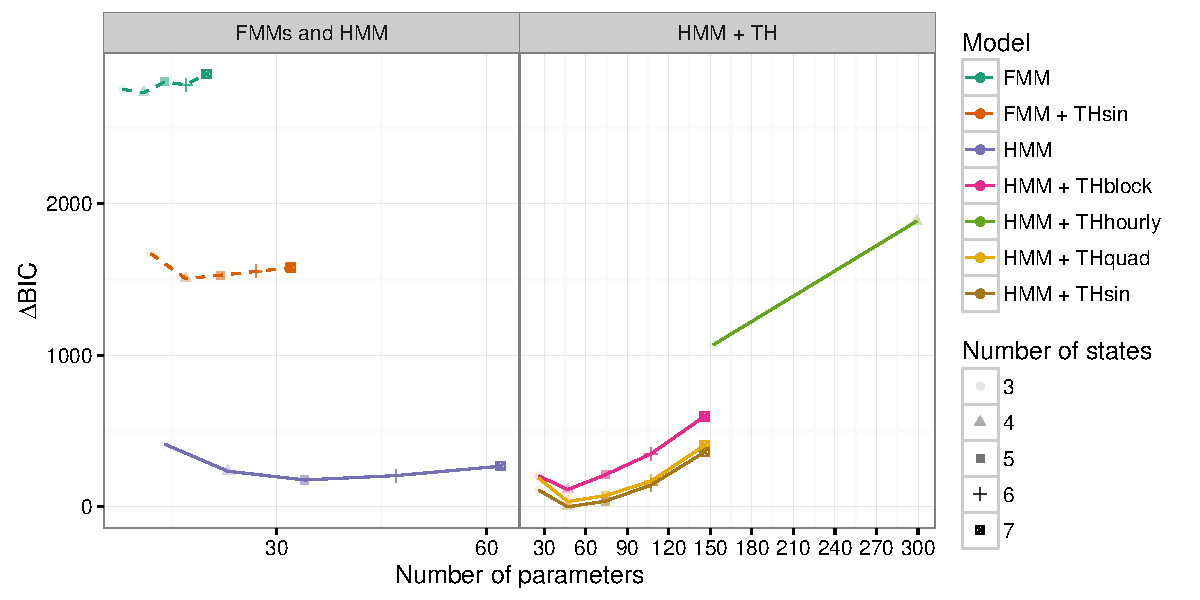
\includegraphics[width=\maxwidth]{figure/adj_BIC_comparisons2-1} \caption{Cat 2: Comparison of adjusted BIC for all HMM transition complexities. The left panel shows homogeneous FMM, heterogeneous FMM (with a sinusoidal prior) and homogeneous HMM. The right panel shows HMMs with different temporal transitions. Dashed lines represents FMMs and solid lines represents HMMs.}\label{fig:adj_BIC_comparisons2}
\end{figure}


\end{knitrout}

\clearpage

\begin{knitrout}
\definecolor{shadecolor}{rgb}{0.969, 0.969, 0.969}\color{fgcolor}\begin{figure}
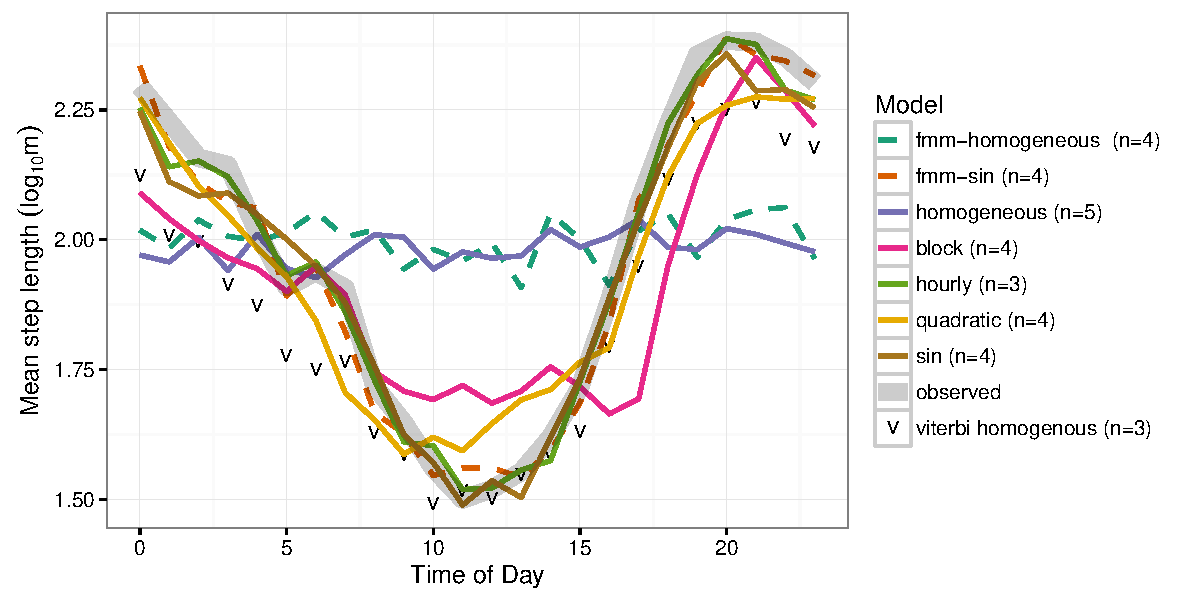
\includegraphics[width=\maxwidth]{figure/avg_step_length_by_time2-1} \caption{Cat 2: Comparison of average step-length by time of day out of sample predictions for BIC-optimal state FMMs (dashed line) and HMMs (solid lines) of different transition complexities. Gray highlight indicate the observed average step length from panther and "V" points represents Viterbi predictions (within sample) of a three-state homogeneous transition HMM.}\label{fig:avg_step_length_by_time2}
\end{figure}


\end{knitrout}

\clearpage

\begin{knitrout}
\definecolor{shadecolor}{rgb}{0.969, 0.969, 0.969}\color{fgcolor}\begin{figure}
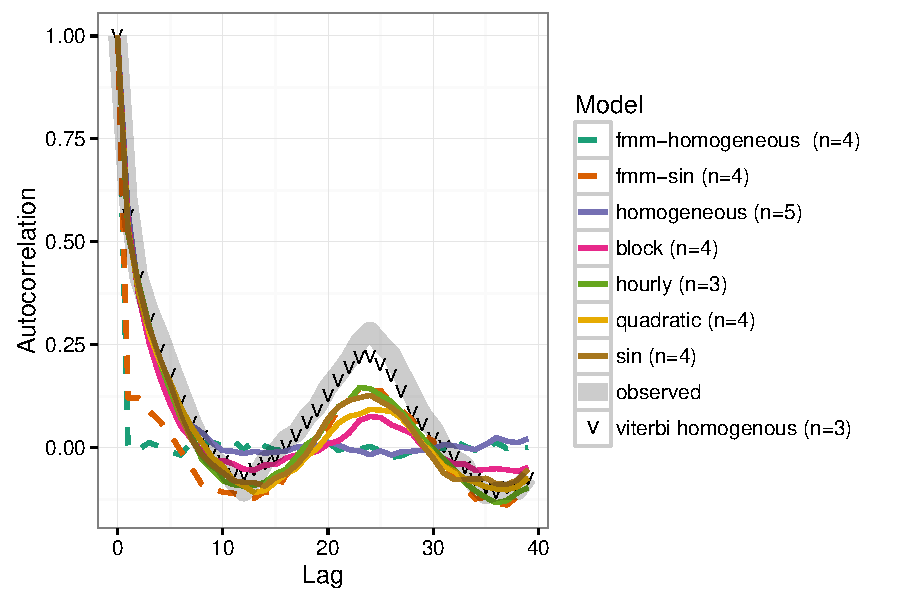
\includegraphics[width=\maxwidth]{figure/acf_plot2-1} \caption{Cat 2: Comparison of out of sample predictions autocorrelations for BIC-optimal state FMMs (dashed line) and HMMs (solid lines) of different transition complexities. Gray highlight indicate the observed average step length from panther and "V" points represents Viterbi predictions (within sample) of a three-state homogeneous transition HMM.}
\end{figure}


\end{knitrout}


\clearpage
%cat14

\begin{knitrout}
\definecolor{shadecolor}{rgb}{0.969, 0.969, 0.969}\color{fgcolor}\begin{figure}
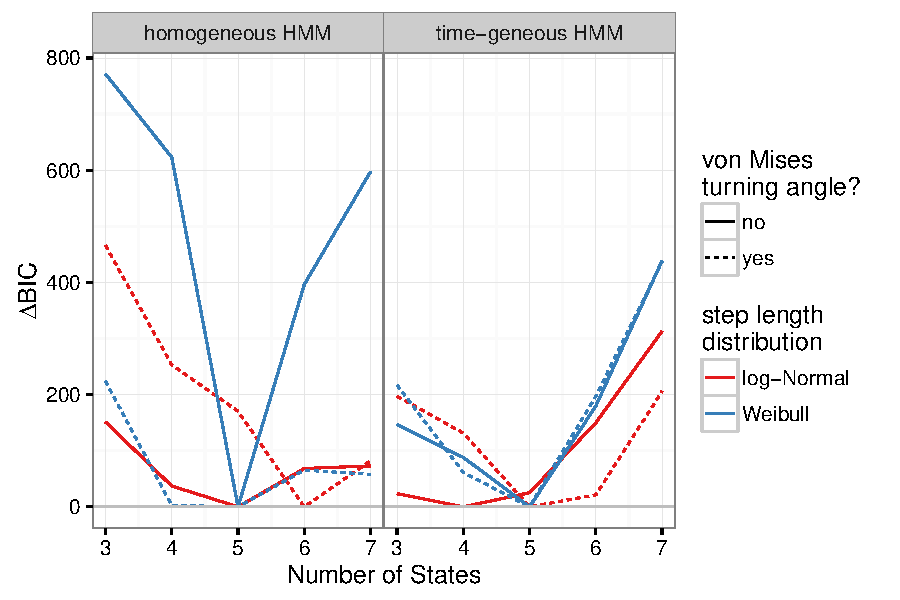
\includegraphics[width=\maxwidth]{figure/BICred_plot14-1} \caption{This figure mataches Figure A1, but for Cat 14.}\label{fig:BICred_plot14}
\end{figure}


\end{knitrout}


\clearpage

\begin{knitrout}
\definecolor{shadecolor}{rgb}{0.969, 0.969, 0.969}\color{fgcolor}\begin{figure}
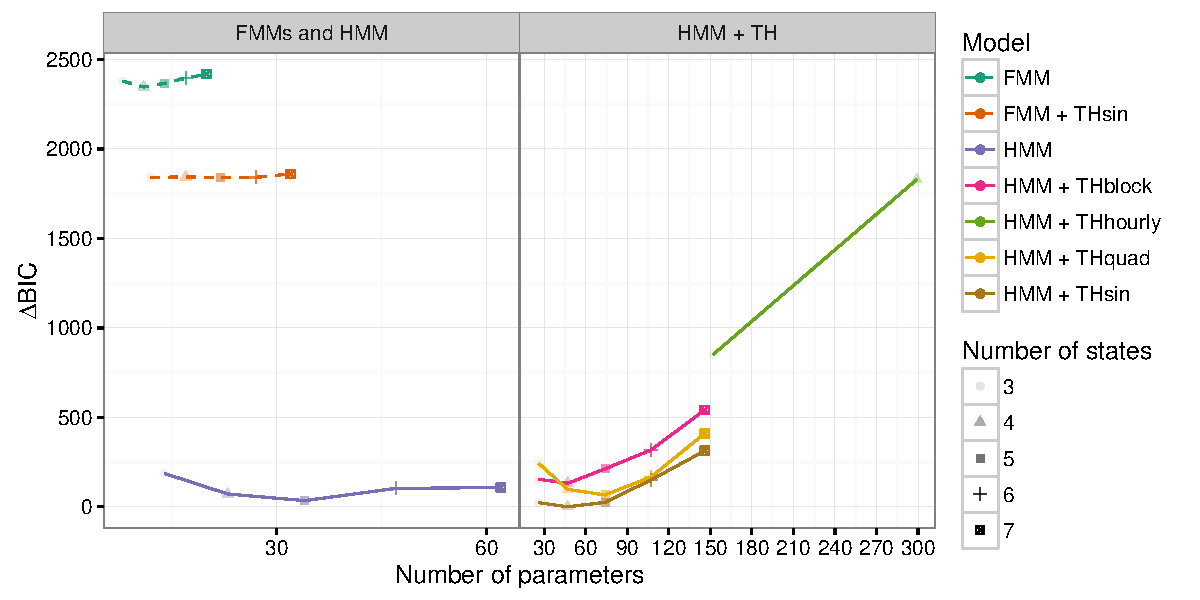
\includegraphics[width=\maxwidth]{figure/adj_BIC_comparisons14-1} \caption{This figure mataches Figure A2, but for Cat 14.}\label{fig:adj_BIC_comparisons14}
\end{figure}


\end{knitrout}

\clearpage

\begin{knitrout}
\definecolor{shadecolor}{rgb}{0.969, 0.969, 0.969}\color{fgcolor}\begin{figure}
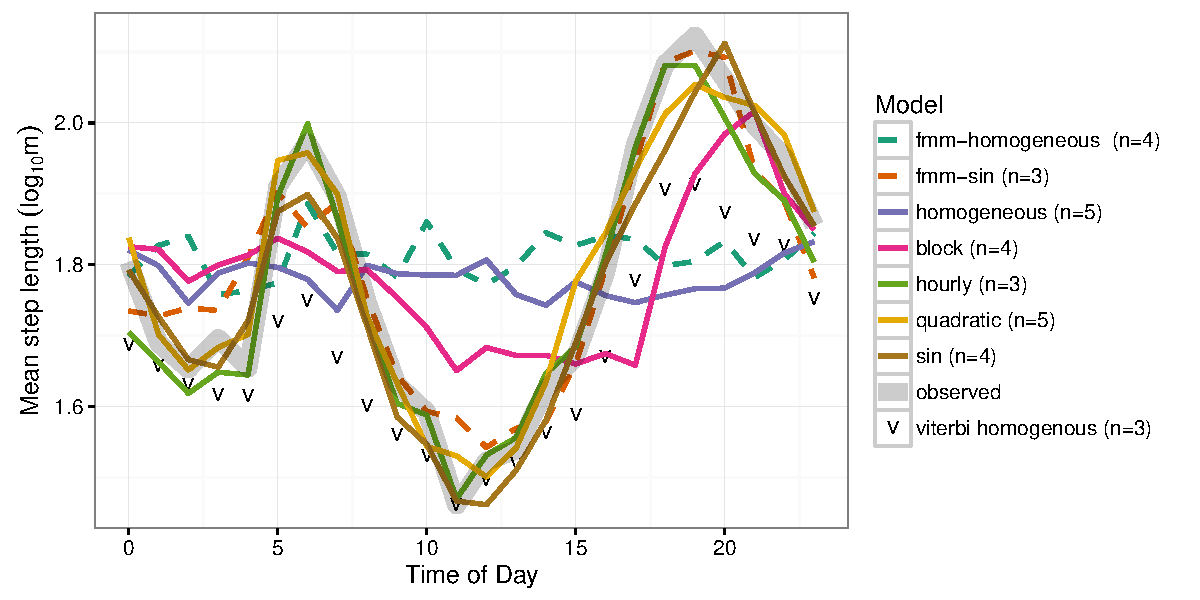
\includegraphics[width=\maxwidth]{figure/avg_step_length_by_time14-1} \caption{This figure mataches Figure A3, but for Cat 14.}\label{fig:avg_step_length_by_time14}
\end{figure}


\end{knitrout}

\clearpage

\begin{knitrout}
\definecolor{shadecolor}{rgb}{0.969, 0.969, 0.969}\color{fgcolor}\begin{figure}
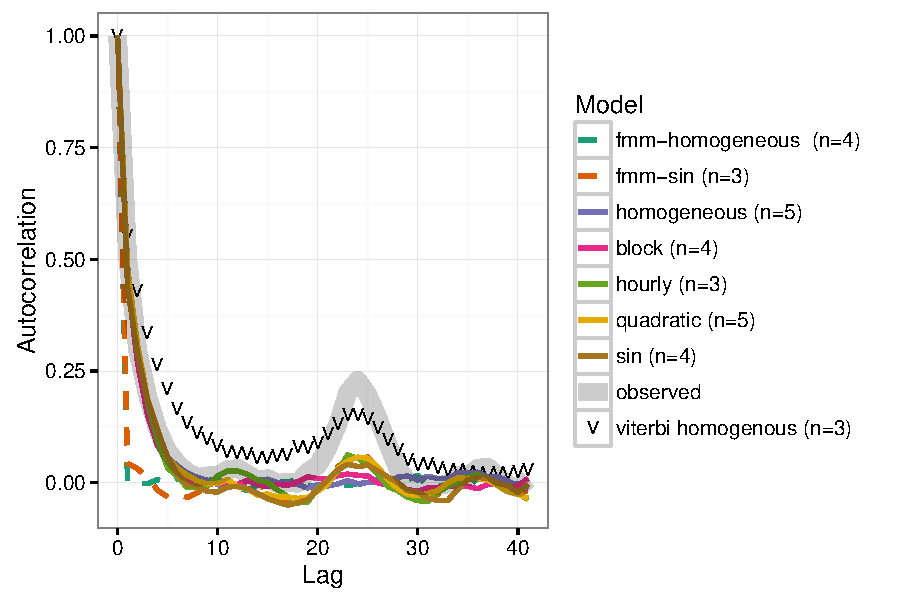
\includegraphics[width=\maxwidth]{figure/acf_plot14-1} \caption{This figure mataches Figure A4, but for Cat 14.}\label{fig:acf_plot14}
\end{figure}


\end{knitrout}

\clearpage
%cat15

\begin{knitrout}
\definecolor{shadecolor}{rgb}{0.969, 0.969, 0.969}\color{fgcolor}\begin{figure}
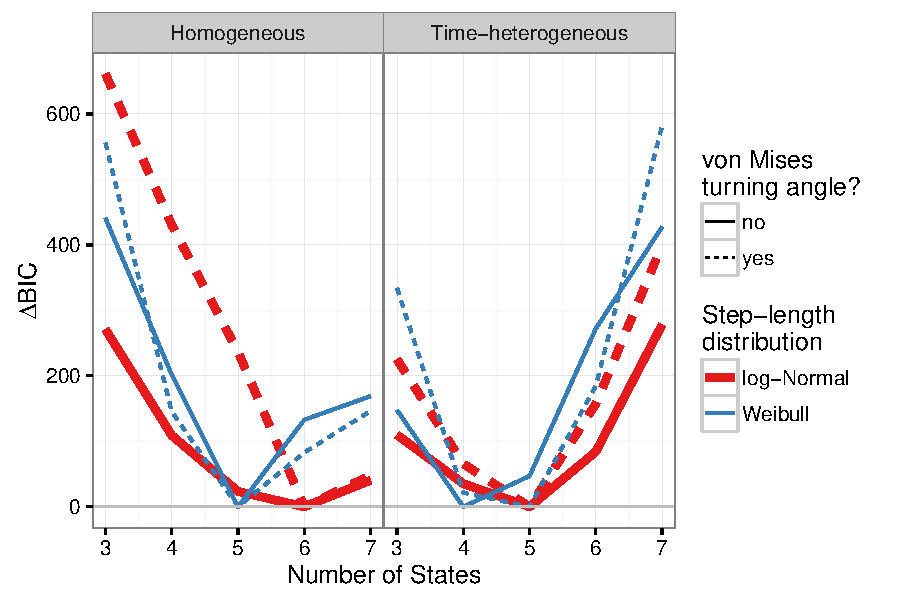
\includegraphics[width=\maxwidth]{figure/BICred_plot15-1} \caption{This figure mataches Figure A1, but for Cat 15.}\label{fig:BICred_plot15}
\end{figure}


\end{knitrout}


\clearpage

\begin{knitrout}
\definecolor{shadecolor}{rgb}{0.969, 0.969, 0.969}\color{fgcolor}\begin{figure}
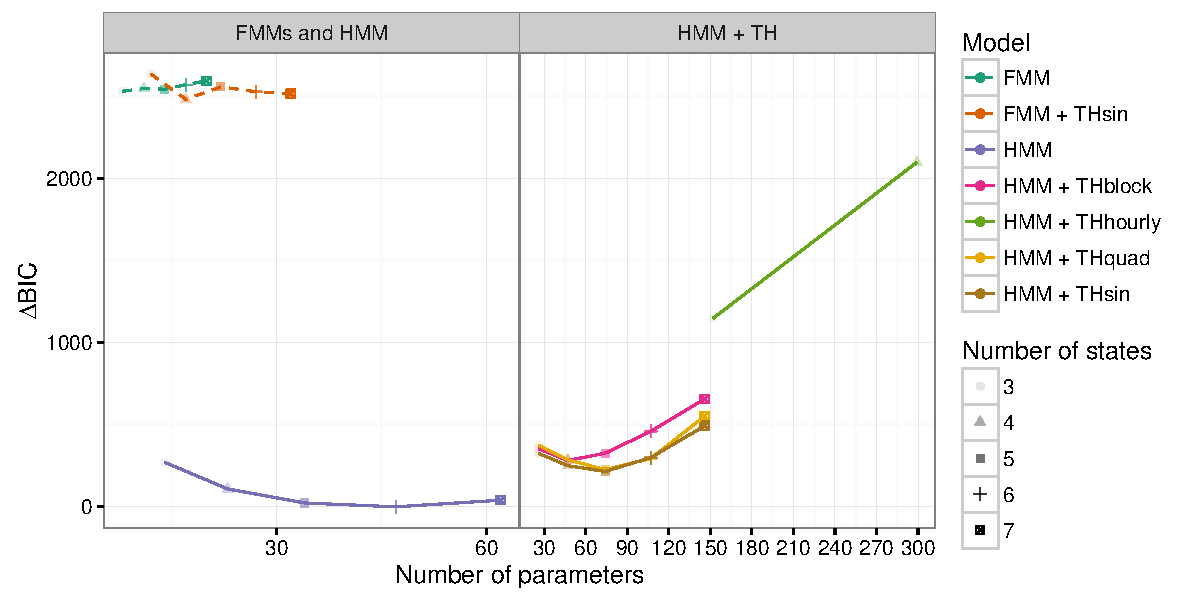
\includegraphics[width=\maxwidth]{figure/adj_BIC_comparisons15-1} \caption{This figure mataches Figure A2, but for Cat 15.}\label{fig:adj_BIC_comparisons15}
\end{figure}


\end{knitrout}

\clearpage

\begin{knitrout}
\definecolor{shadecolor}{rgb}{0.969, 0.969, 0.969}\color{fgcolor}\begin{figure}
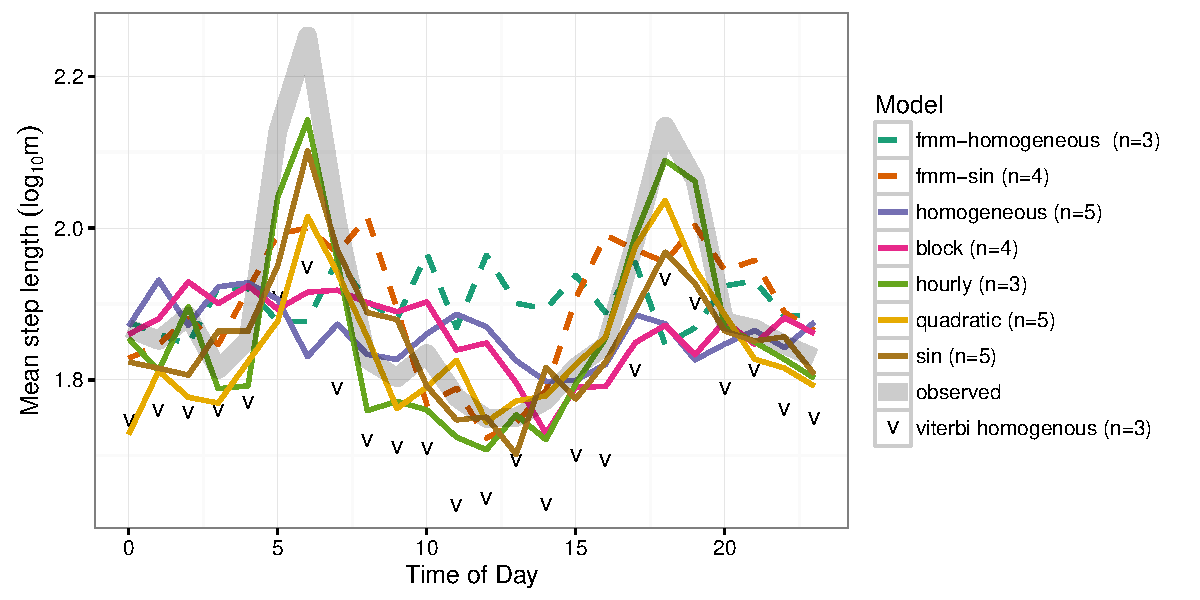
\includegraphics[width=\maxwidth]{figure/avg_step_length_by_time15-1} \caption{This figure mataches Figure A3, but for Cat 15.}\label{fig:avg_step_length_by_time15}
\end{figure}


\end{knitrout}

\clearpage

\begin{knitrout}
\definecolor{shadecolor}{rgb}{0.969, 0.969, 0.969}\color{fgcolor}\begin{figure}
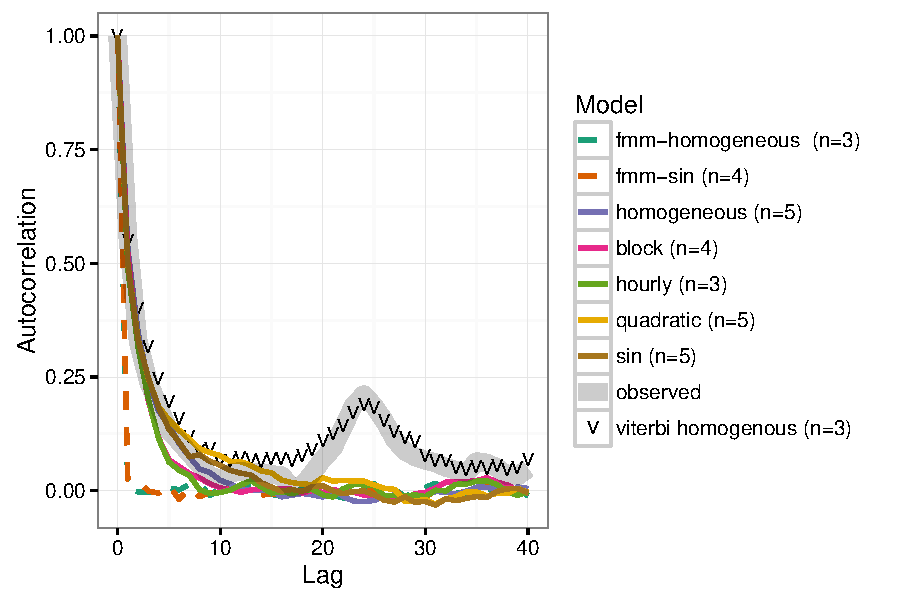
\includegraphics[width=\maxwidth]{figure/acf_plot15-1} \caption{This figure mataches Figure A4, but for Cat 15.}\label{fig:acf_plot15}
\end{figure}

\clearpage

\end{knitrout}
\bibliographystyle{bmc-mathphys} % Style BST file (bmc-mathphys, vancouver, spbasic).
\bibliography{panthers}

\end{document}
